\chapter{Pipelining}
\lectlink{https://imperial.cloud.panopto.eu/Panopto/Pages/Viewer.aspx?id=463efb5a-dd91-4592-9460-af2a010e5ba3}{Chapter 1 - Part 2: Pipelines}
\begin{definitionbox}{MIPS/Microprocessor without Interlocked Pipelined Stages}
    MIPS is a reduced instruction set (RISC) architecture originally developed for the \href{https://en.wikipedia.org/wiki/R2000_microprocessor}{R2000 microprocessor}.
    \begin{itemize}
        \item 3 types of instruction layouts
        \item Load-store architecture
        \item Support for floating point arithmetic
    \end{itemize}
\end{definitionbox}

\section{Instruction Layout}
The instructions set architecture (ISA) determines the layout of instructions. Here we consider the mips architecture.
\begin{center}
    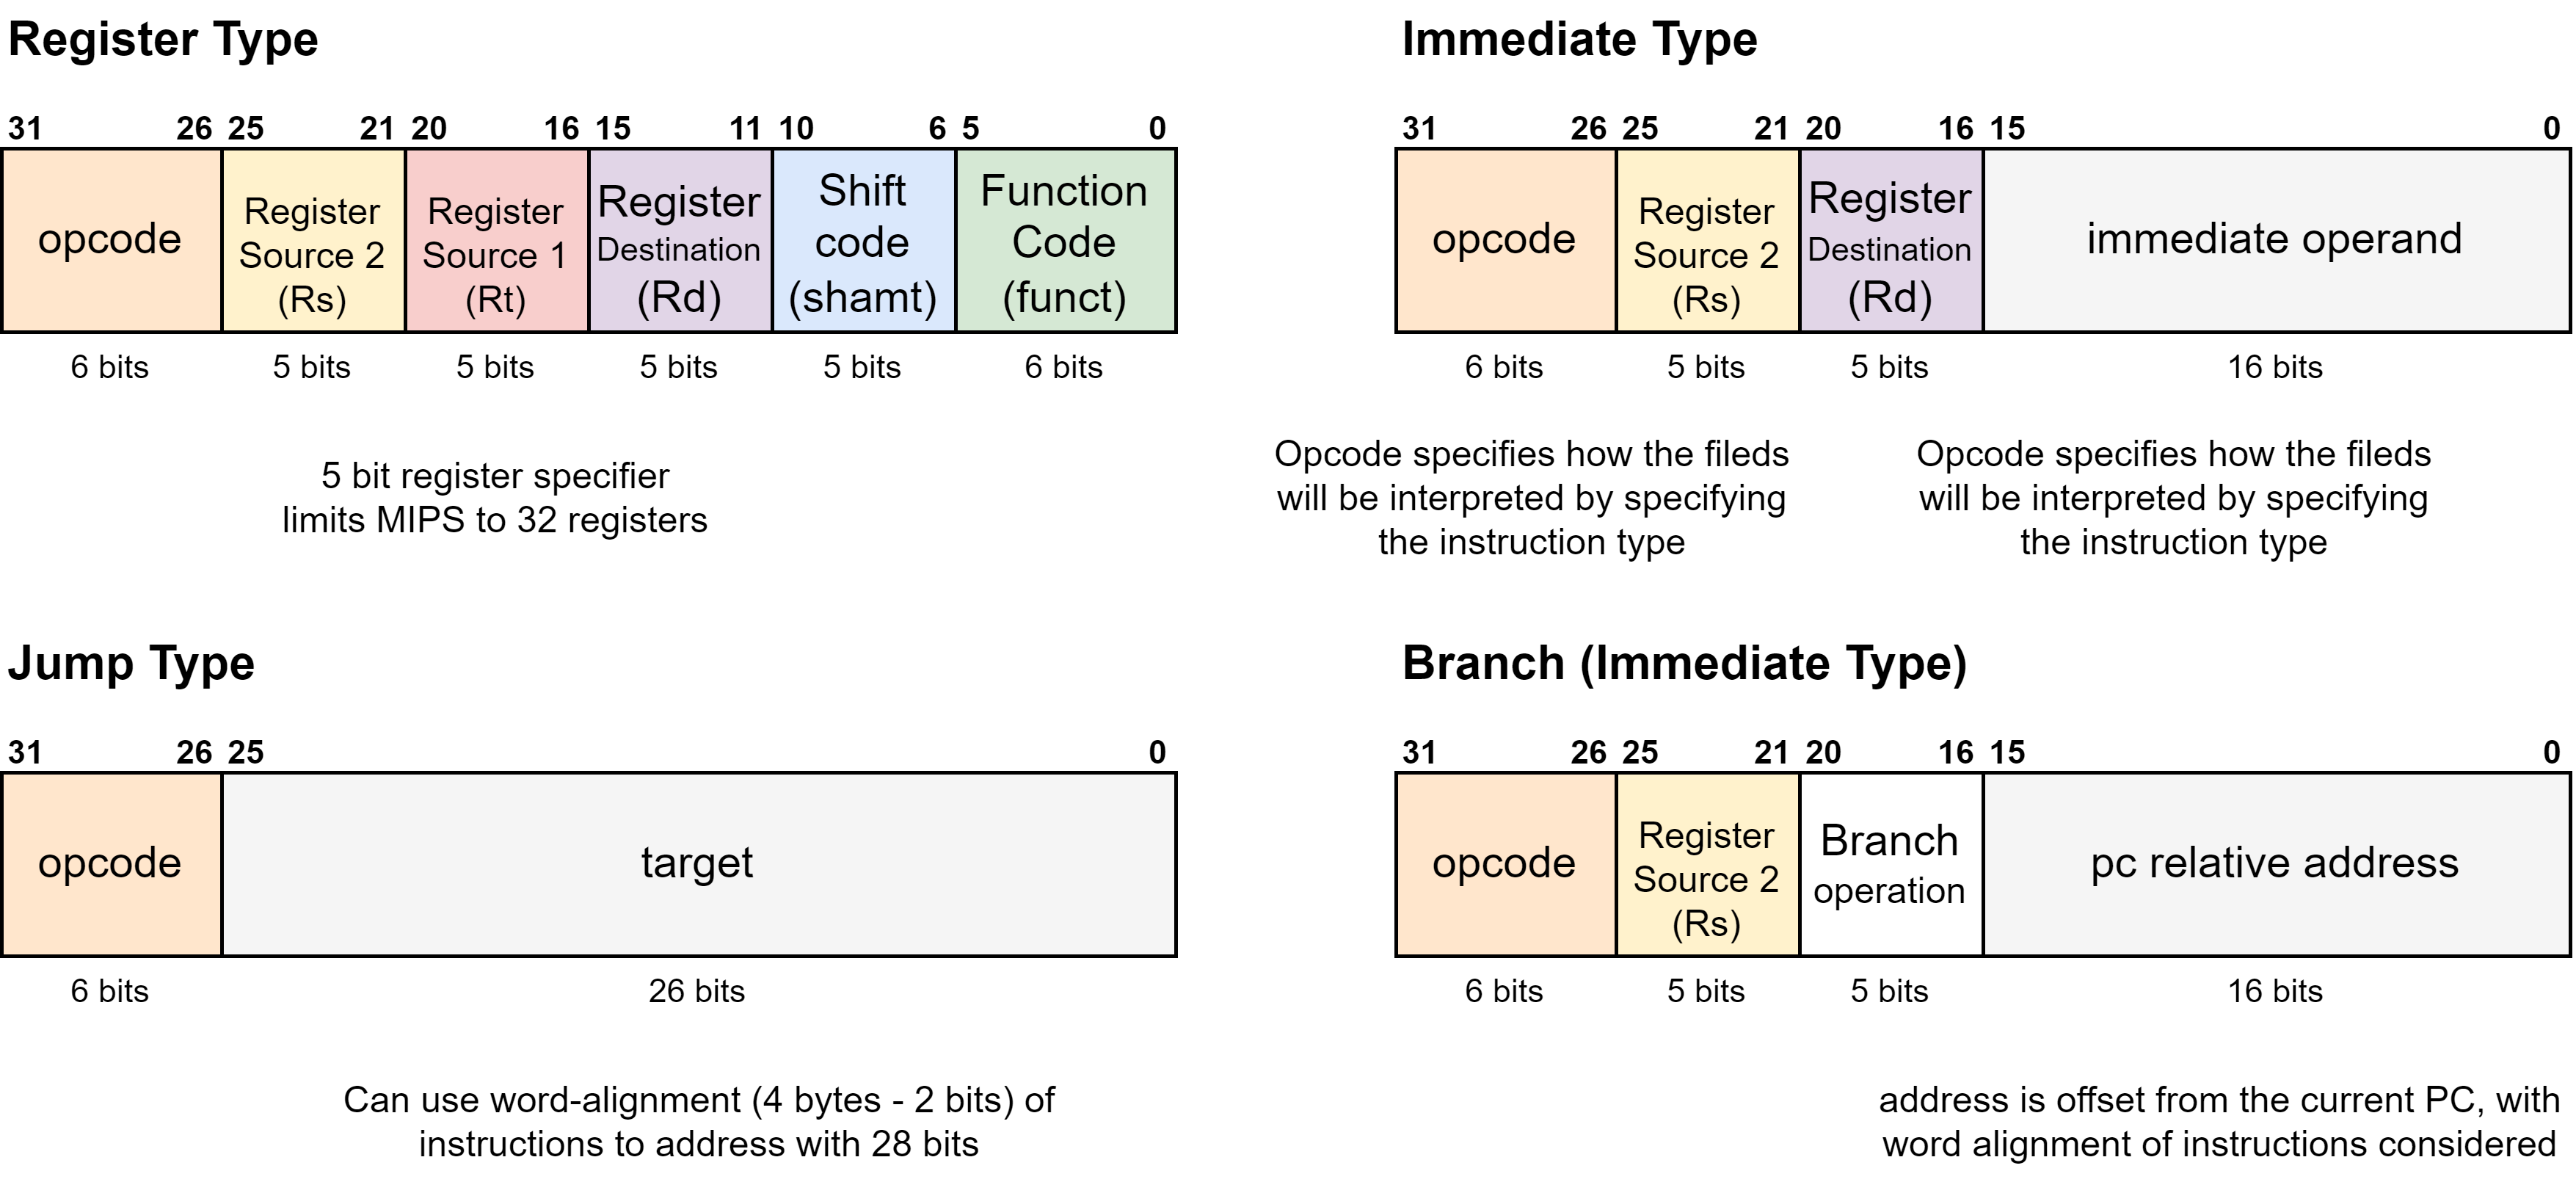
\includegraphics[width=.9\textwidth]{pipelining/images/MIPS_instruction_set.drawio.png}
\end{center}
The size of fields in the instruction layouts determines characteristics such as:
\begin{itemize}
    \item Maximum number of registers
    \item Maximum distance for a conditional jump
    \item Size of immediate operands
    \item Range of addresses that can be used.
\end{itemize}
\begin{sidenotebox}{MIPS Assembly}
    A basic guide listing of mips instructions can be found here \href{https://www.dsi.unive.it/~gasparetto/materials/MIPS_Instruction_Set.pdf}{Basic MIPS instructions}.
\end{sidenotebox}

\section{Pipeline Structure}
\begin{center}
    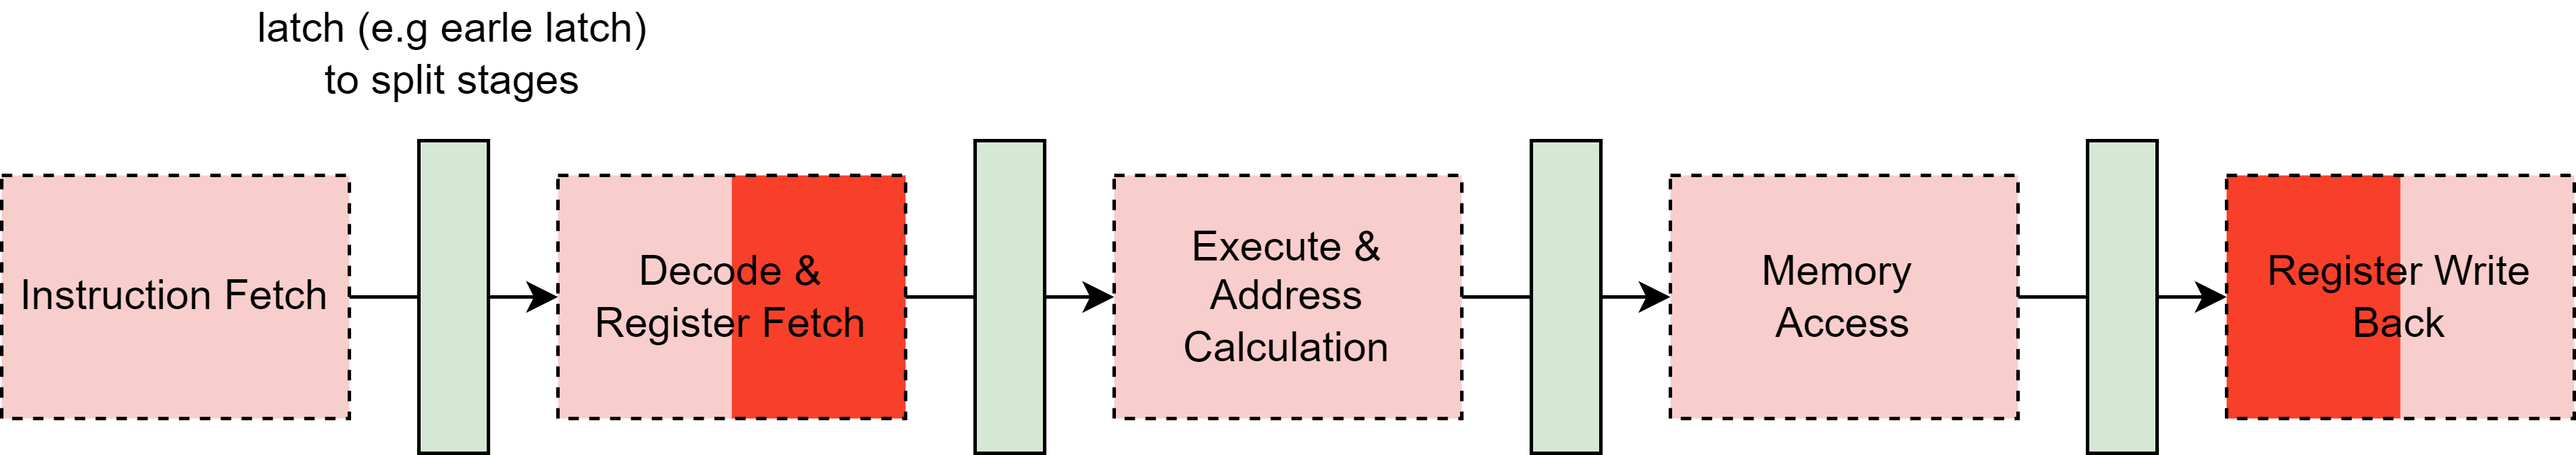
\includegraphics[width=.8\textwidth]{pipelining/images/MIPS_pipeline_stages.drawio.png}
\end{center}
\begin{itemize}
    \item Execution of an instruction is split into stages
    \item Throughput is potentially increased by factor $\sfrac{1}{\text{number of stages}}$ (idealistically)
    \item All stages work on an instruction simultaneously/in parallel (very little extra hardware required for the speedup advantage)
\end{itemize}
The speedup is reduced by
\begin{itemize}
    \item Latency increased due to latches
    \item Pipeline rate limited by slowest stage (unbalanced stages / fragmentation)
    \item Time required to fill and drain the pipeline.
    \item Pipeline hazards which result in stalls (unable to dispatch another instruction in a given cycle).
\end{itemize}

\section{Pipeline Hazards}
\subsection{Structural Hazard}
\begin{definitionbox}{Structural Hazard}
    Where hardware is unable to support a combination of instructions.
\end{definitionbox}
Multiple pipeline stages may need to access the same hardware resources:
\begin{itemize}
    \item Register file (register operand fetch and register write back)
    \item Access to memory (RAM port in older machines, cache (SRAM) now)
\end{itemize}
\begin{examplebox}{Not enough ports!}
    Given basic pipeline structure above, what structural hazard could occur between \textit{Memory Access} and \textit{instruction fetch} if there is only one RAM port?
    \tcblower
    No instruction can be fetched when the \textit{Memory Access} stage is filled, this results in a stall. 
    \\
    \\ The maximum potential speedup for a 5 stage pipeline is $5\times$, however due to the stalls we can see a recurring pattern:
    \begin{center}
        \begin{tabular}{r c c c c c c c}
            \textbf{Cycle:} & $6n$ & $6n+1$ & $6n+2$ & $6n+3$ & $6n+4$ & $6n+5$ \\
            \textbf{Instructions:} & 2 & 2 & 3 & 3 & 3 & 2 \\
        \end{tabular}
    \end{center}
    We would expect a $5\times$ speedup from this pipeline. However we are only getting a $2.5\times$ speedup due to the stalls.

    \begin{center}
        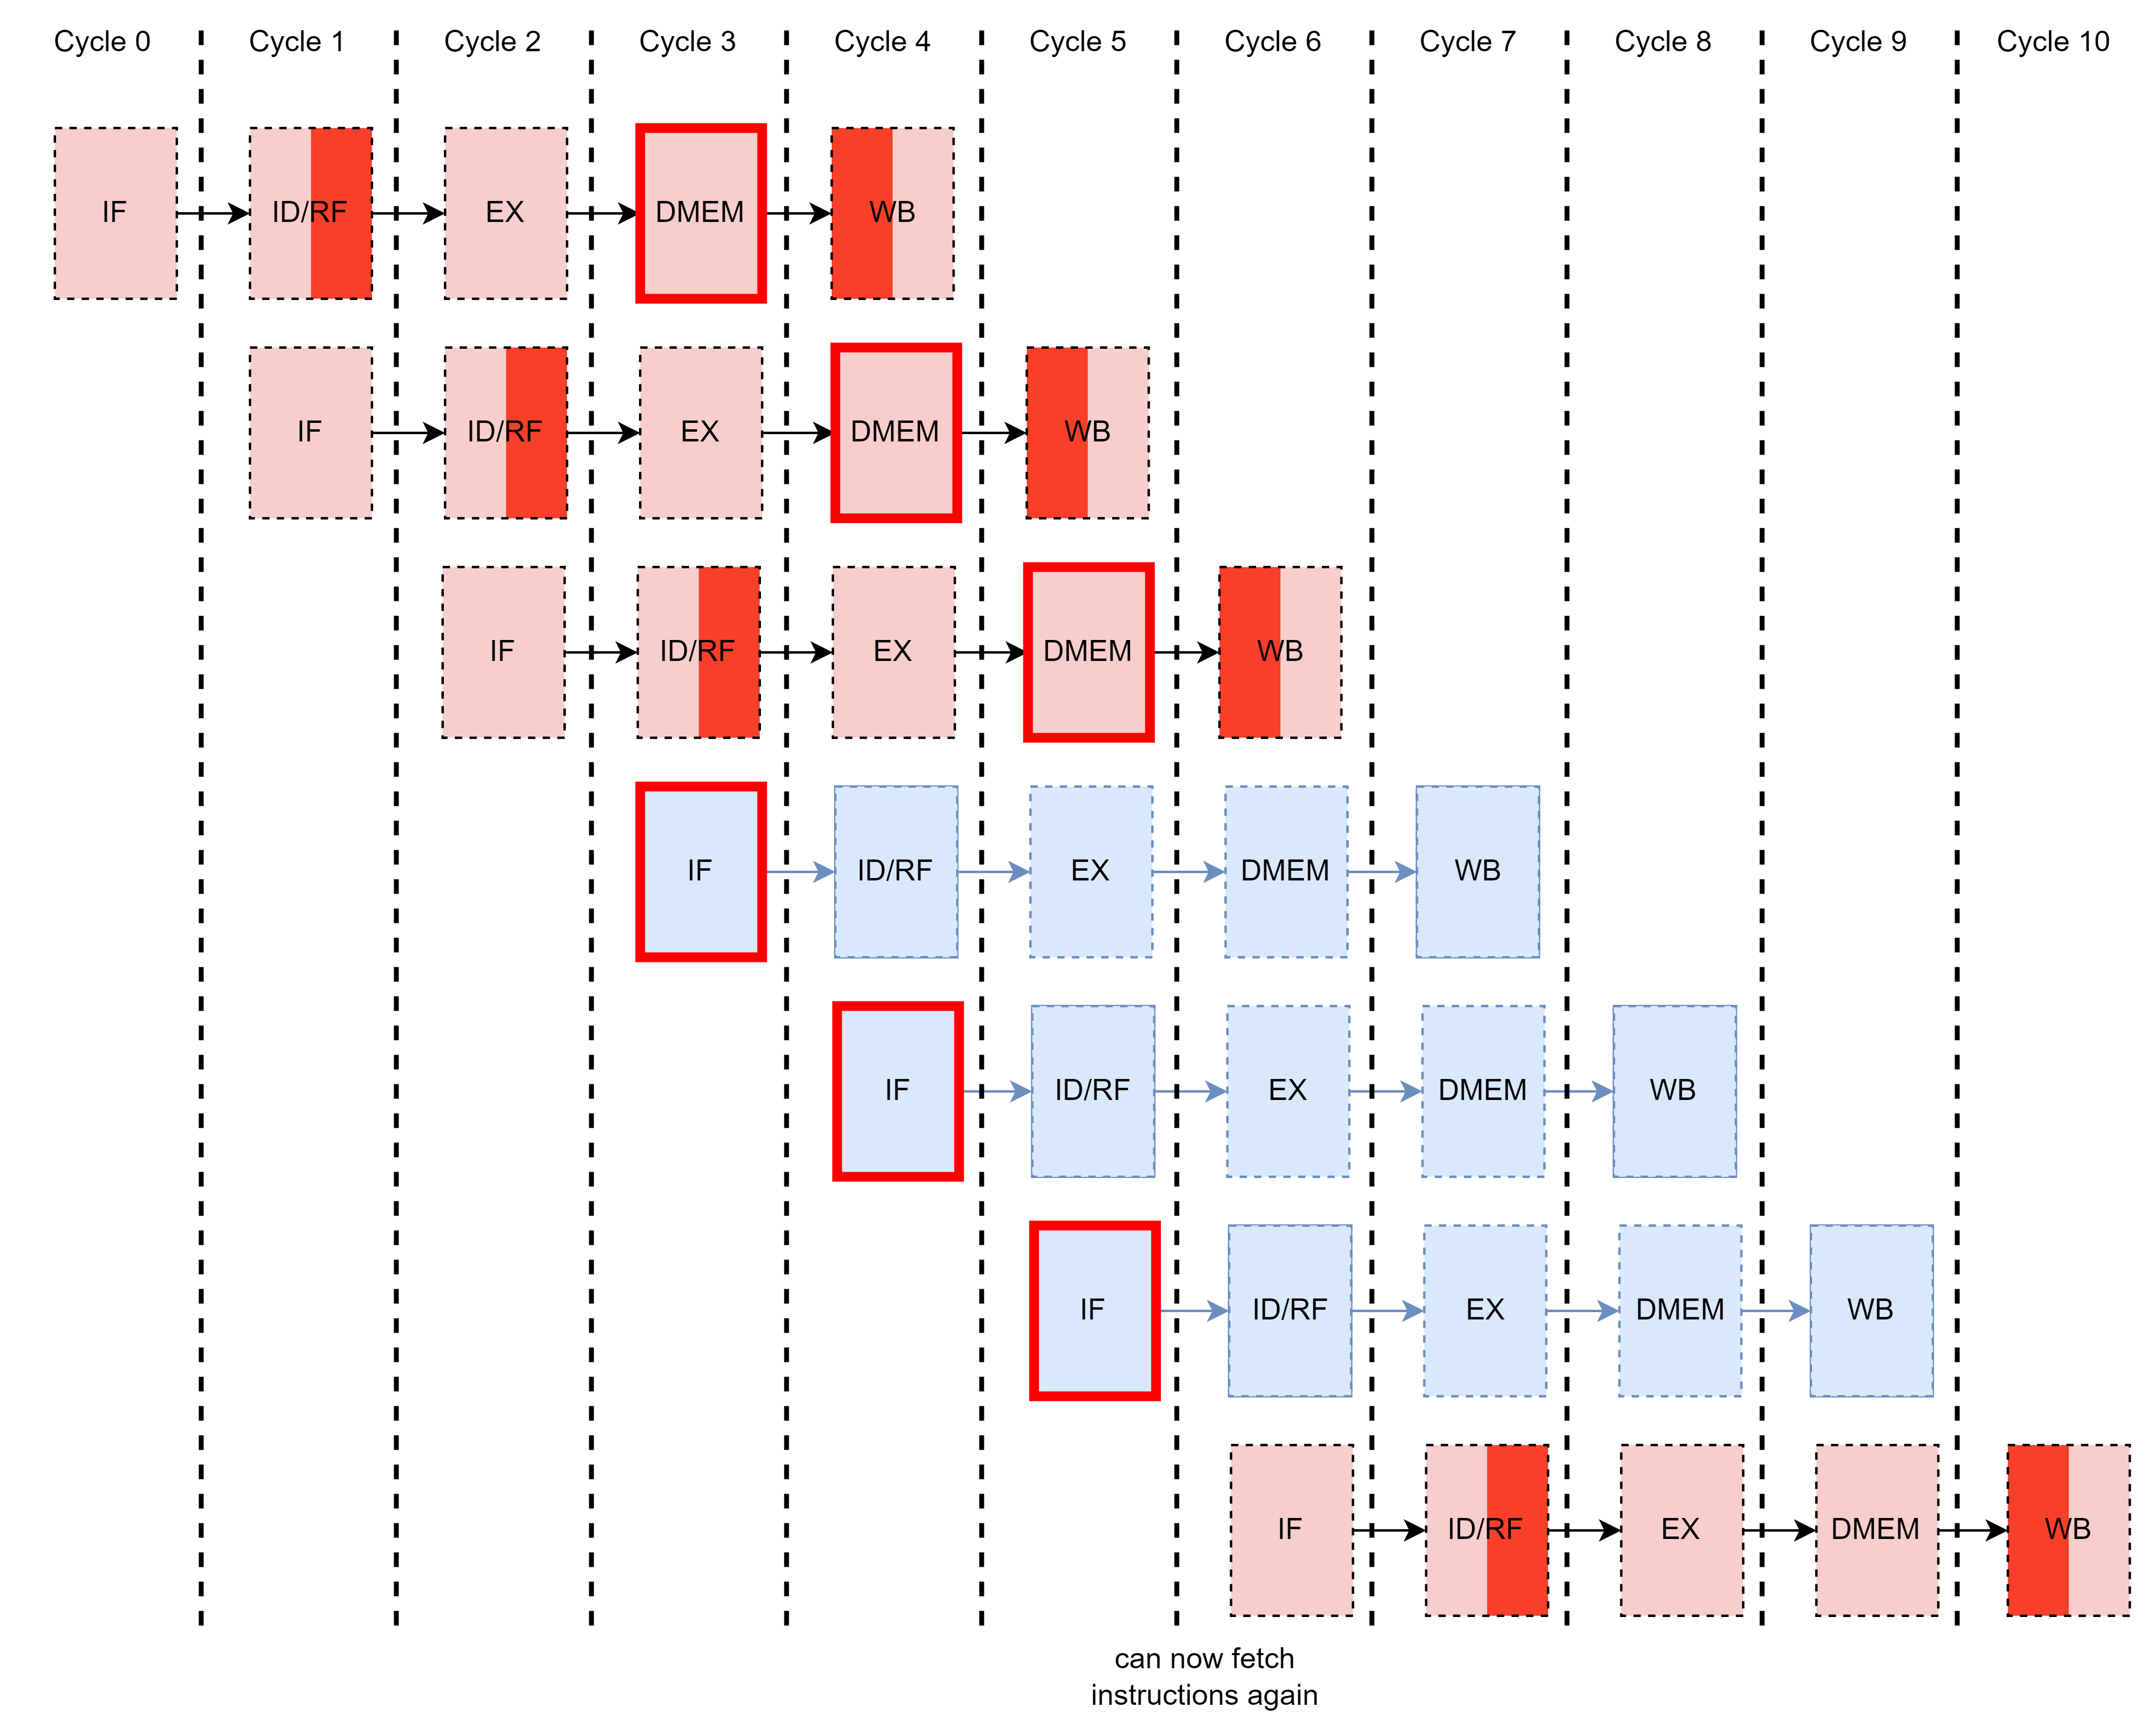
\includegraphics[width=\textwidth]{pipelining/images/example_structural_hazard.drawio.png}
    \end{center}
\end{examplebox}

\subsection{Data Hazard}
\begin{definitionbox}{Data Hazard}
    Instruction is dependent on the result of a prior instruction still in the pipeline.
\end{definitionbox}
Most often caused by a dependency between instructions. 
\begin{definitionbox}{Forwarding Paths}
    Paths between pipeline stages to allow results from previous instructions (not yet written back) to be sent to instructions afterwards that are in the pipeline.
\end{definitionbox}
\subsubsection{Result Used By Many Subsequent Instructions}
\begin{minted}{text}
li    $1, 100      # $1 = 100
addiu $2, $1, 100  # $1 += 100 # here onwards depends on $1
addiu $3, $1, 100  # $1 += 100
addiu $4, $1, 100  # $1 += 100
\end{minted}
\begin{center}
    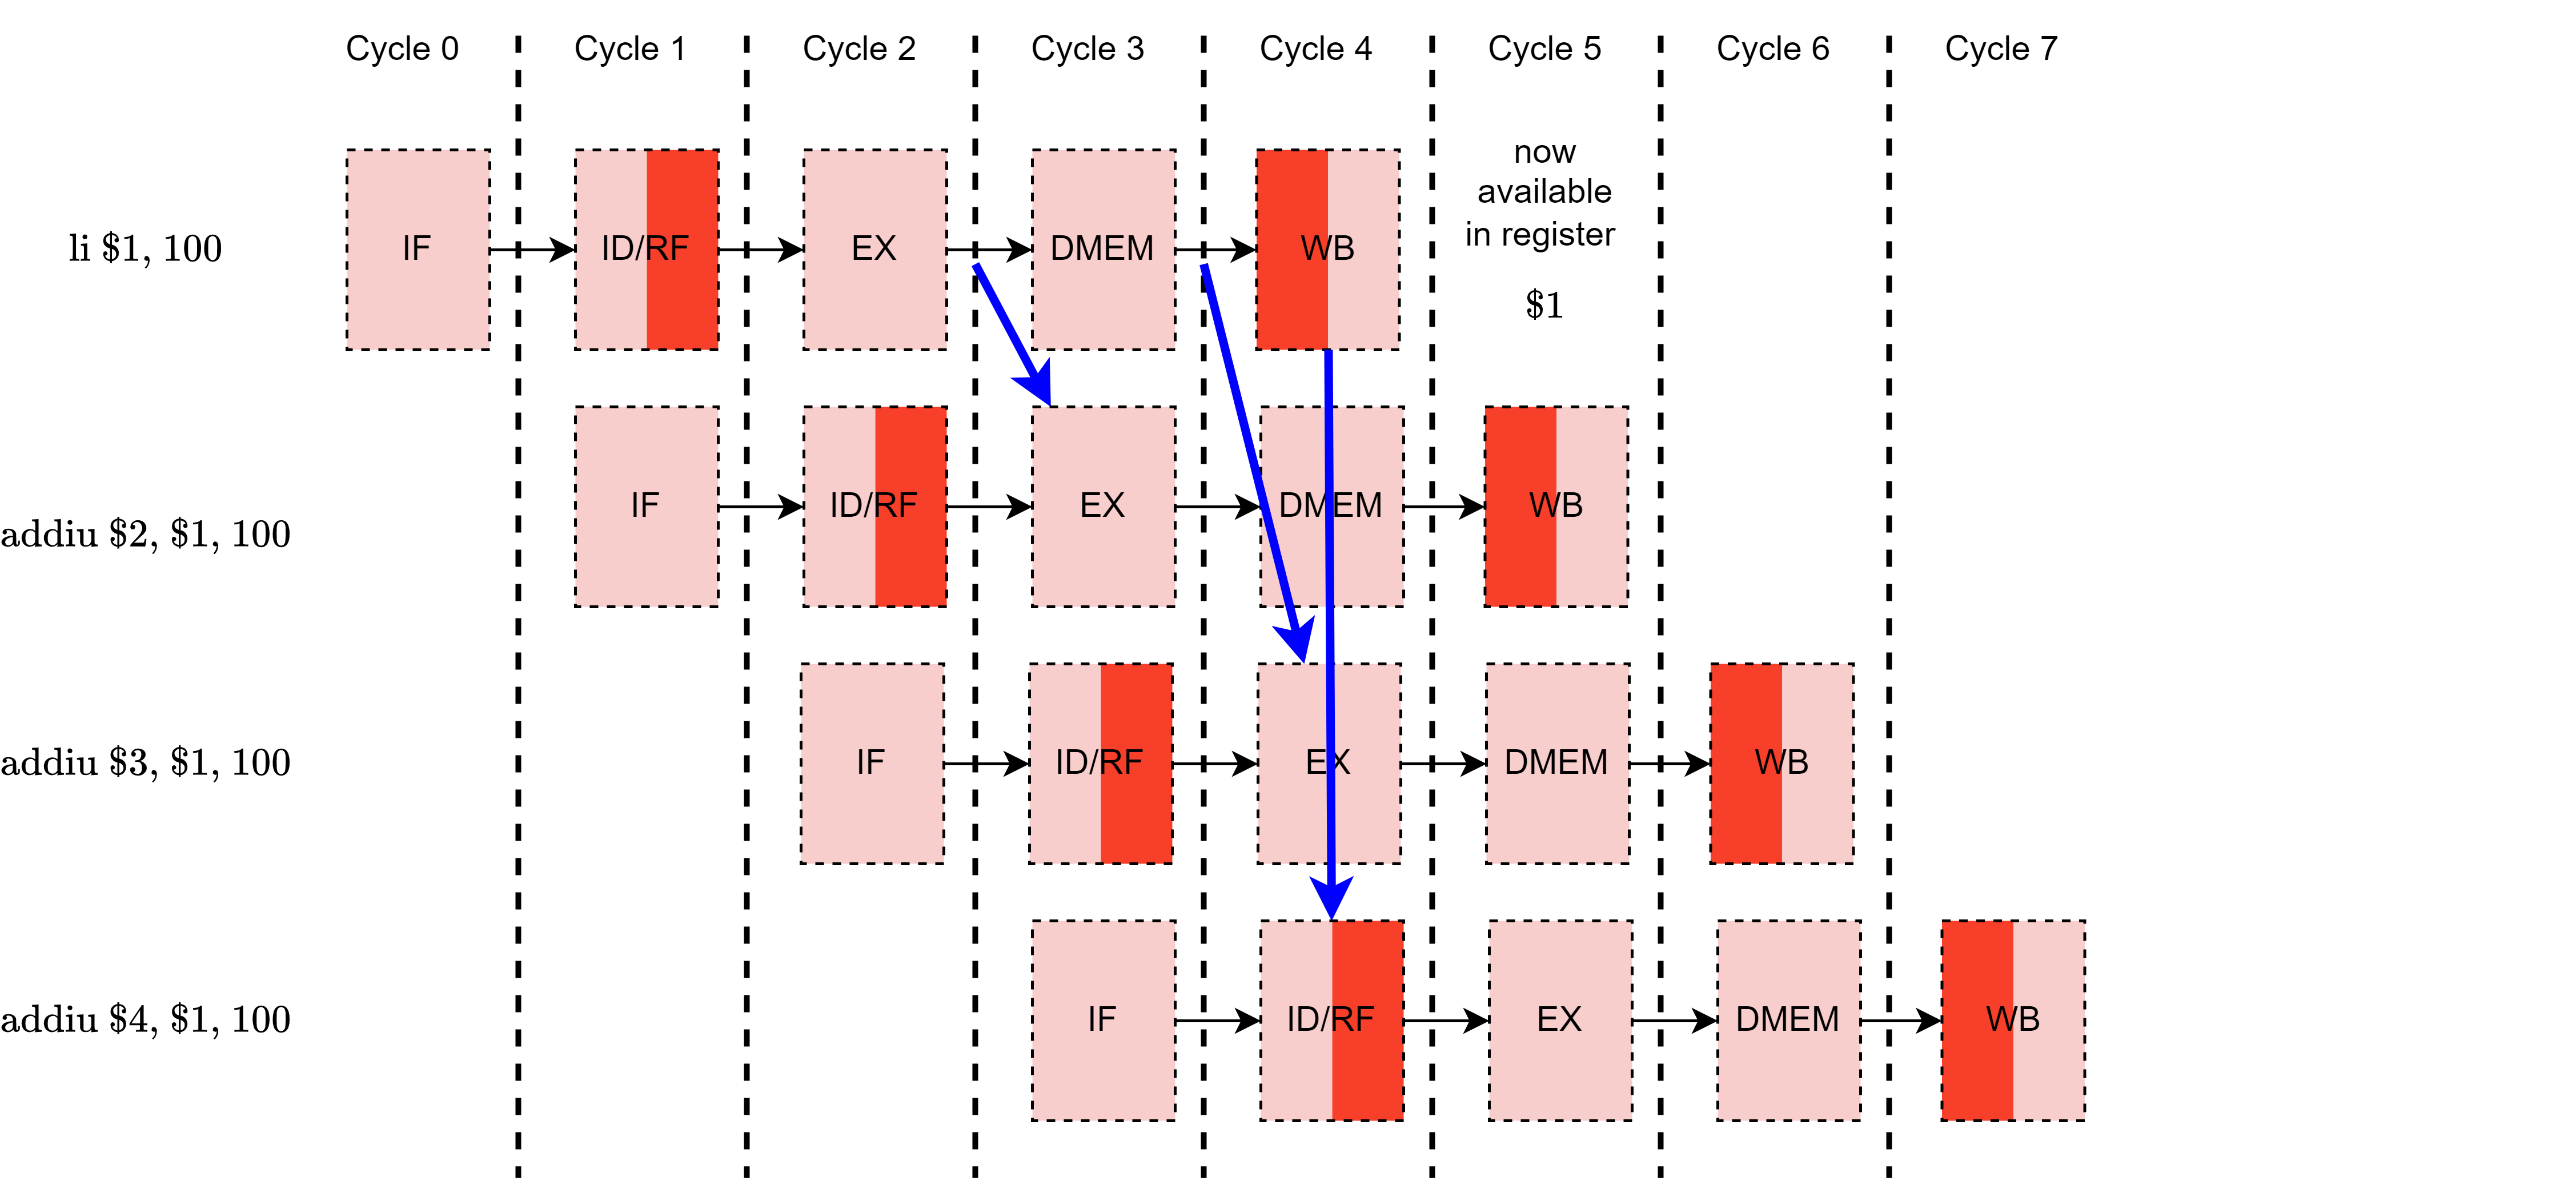
\includegraphics[width=.9\textwidth]{pipelining/images/pipeline_operand_forward_1.drawio.png}
\end{center}

\subsubsection{Chain of Results}
\begin{minted}{text}
li    $1, 100      # $1 = 100
addiu $2, $1, 100  # $1 += 100
addiu $3, $2, 100  # $1 += 100
addiu $4, $3, 100  # $1 += 100
\end{minted}
\begin{center}
    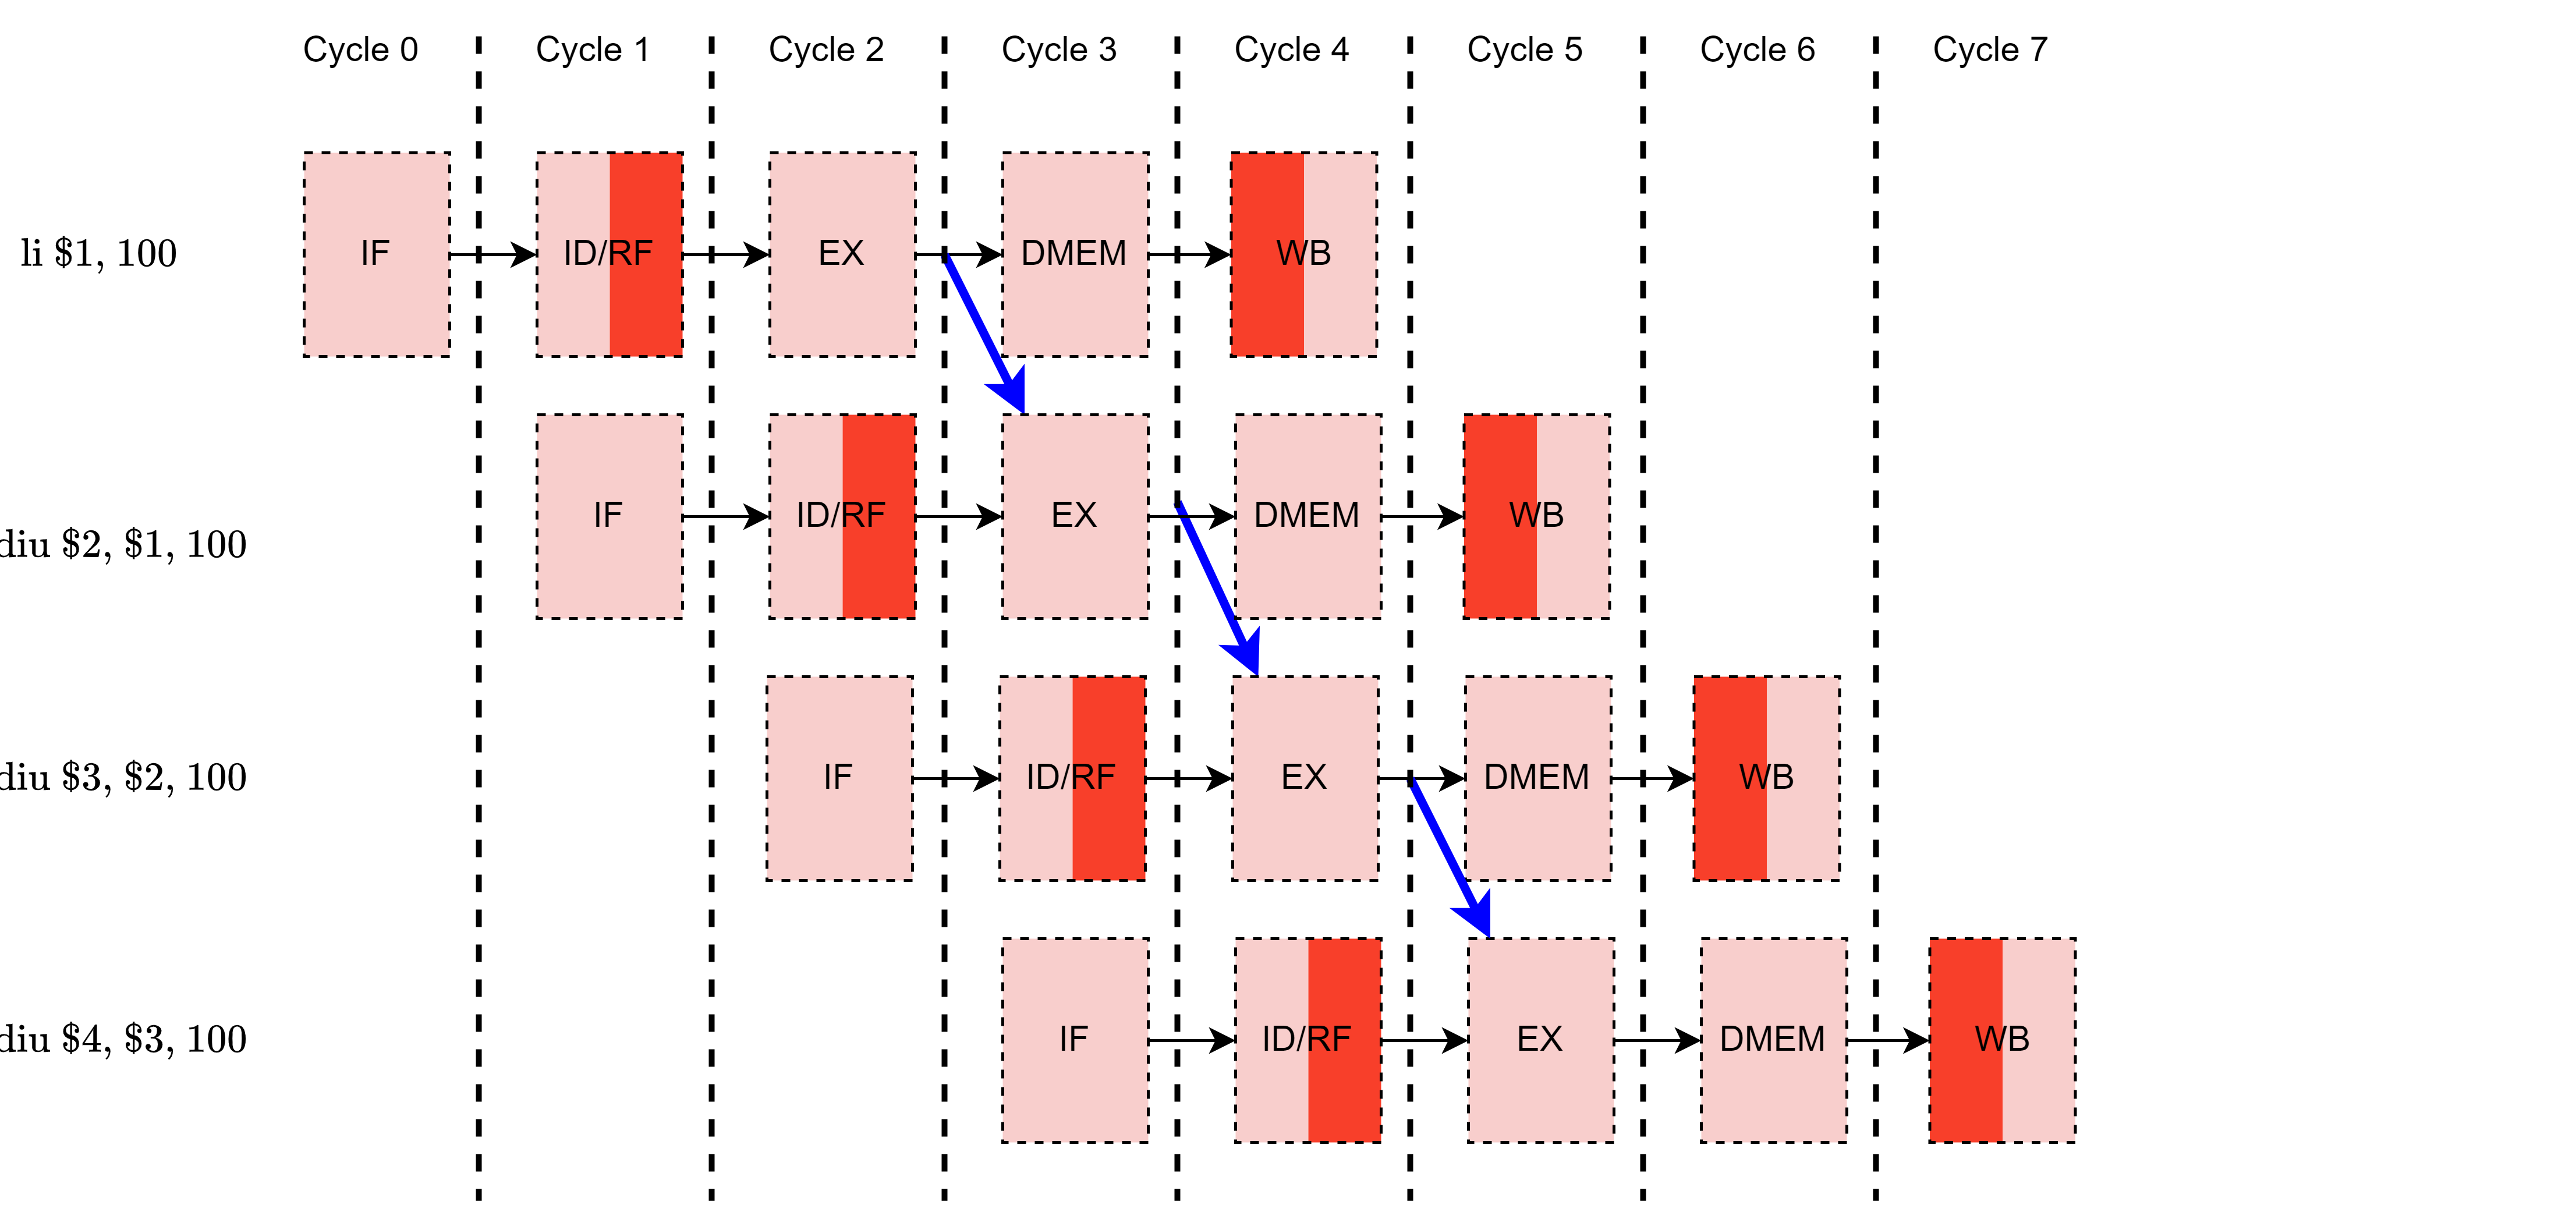
\includegraphics[width=.9\textwidth]{pipelining/images/pipeline_operand_forward_2.drawio.png}
\end{center}
\subsubsection{Data Hazard Despite Forwarding}
Here have a \textit{load to use stall/delay}, forwarding paths will not work here as the memory access stage is 2 stages later than execute (where the instruction is required).
\begin{minted}{text}
lw    $1, 0($2)    # $1 = *($2)
addiu $2, $1, 100  # $1 += 100 
addiu $3, $1, 100  # $1 += 100
addiu $4, $1, 100  # $1 += 100
\end{minted}
\begin{center}
    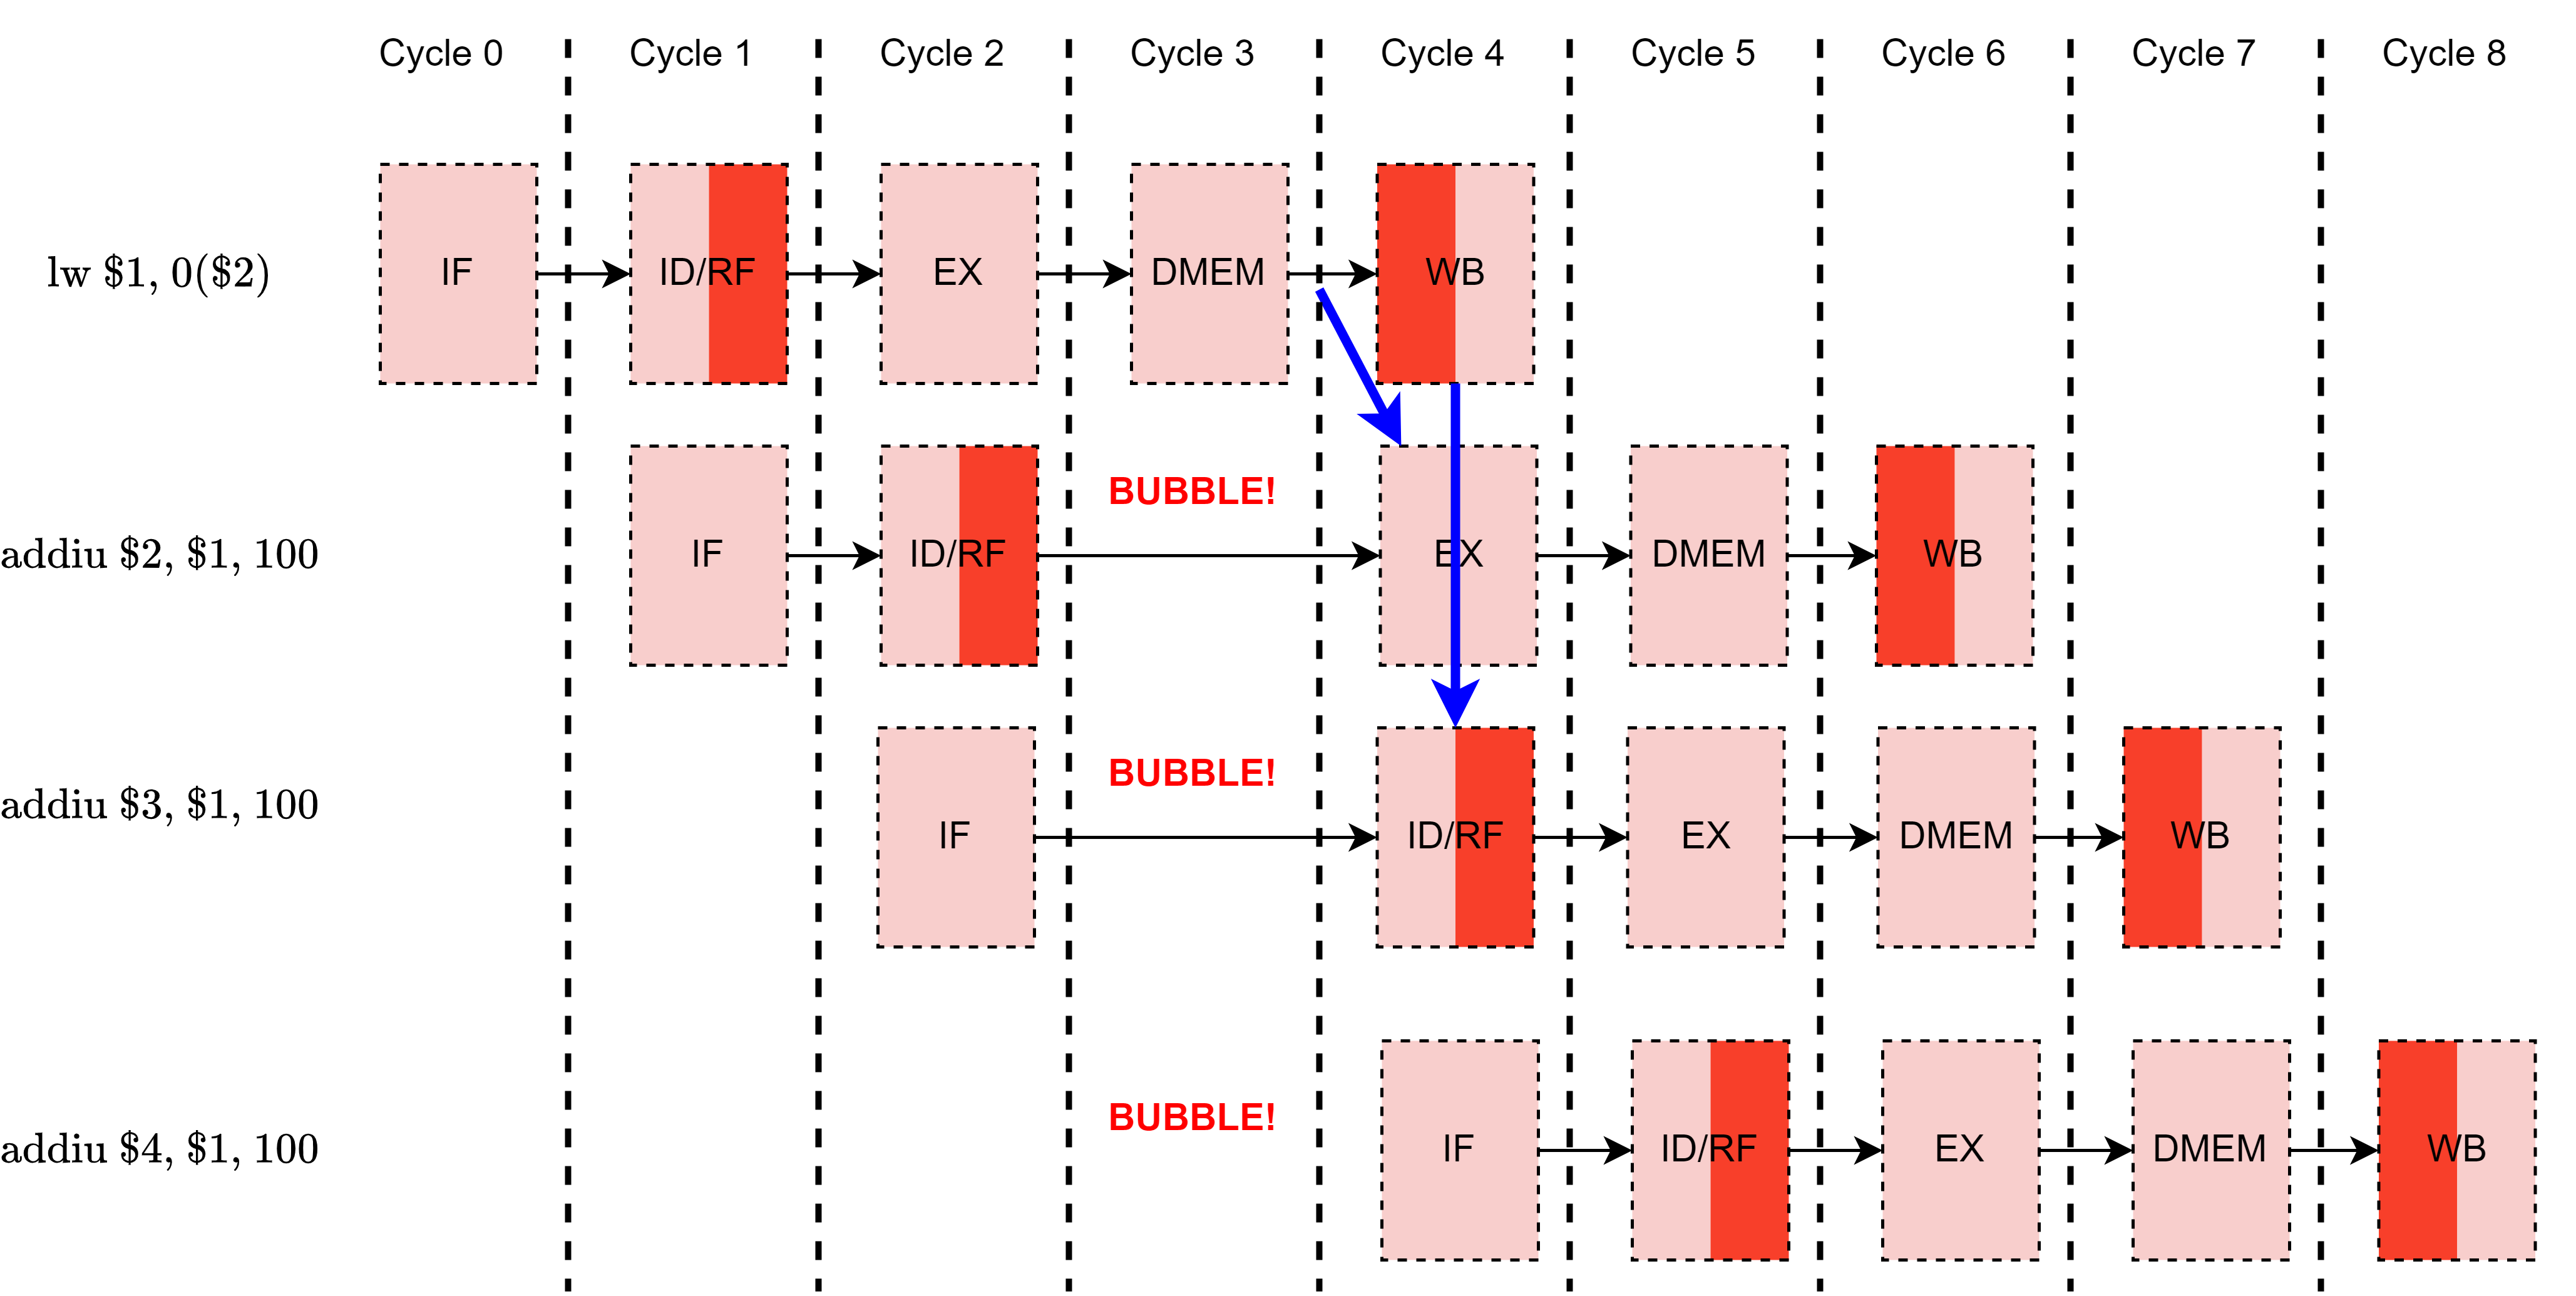
\includegraphics[width=.9\textwidth]{pipelining/images/pipeline_operand_forward_3.drawio.png}
\end{center}
We can attempt to solve this issue using the compiler (e.g reorder instructions to put at least one non-dependent instruction between the load and the use).
\subsubsection{Forwarding Paths}
\subsubsection{Software Scheduling}


\subsection{Control Hazard}
\begin{definitionbox}{Control Hazard}
    A stall created by the delay between getting the result of some branch/jump and fetching the next instruction using that data.
\end{definitionbox}
Instruction fetch (without branch prediction) requires the conditional branch result to be known. Hence the number of stages between instruction fetch and when the branch condition is determined is the size of the stall resulting from a conditional branch.
\begin{itemize}
    \item This is also true for jumps/unconditional branches where the address is provided by some register and arithmetic (e.g jump with offset)
    \item Branch prediction can be done dynamically (in hardware) or statically (specific branch likely, branch unlikely instructions used by compiler).
\end{itemize}
\begin{center}
    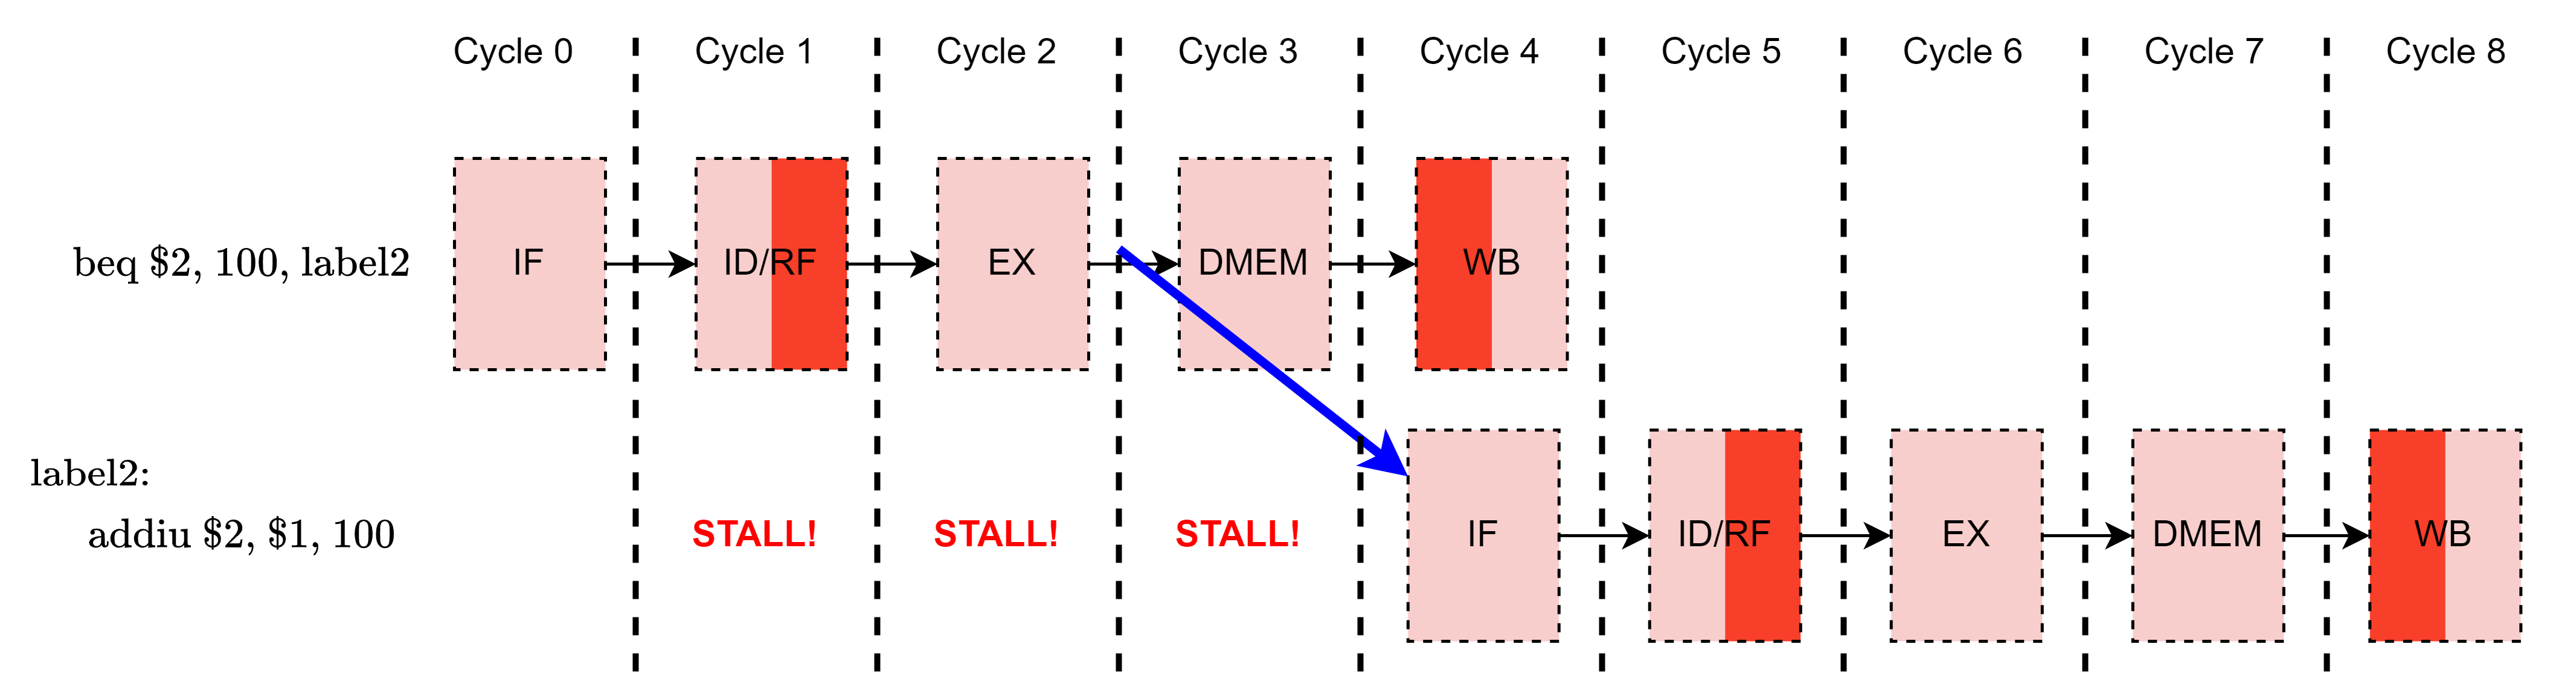
\includegraphics[width=.9\textwidth]{pipelining/images/control_hazard_conditional_branch.drawio.png}
\end{center}

\subsubsection{Early Branch Determination}
To decrease the number of cycles stalled in a branch, we can move the branch determination to earlier in the pipeline.
\begin{itemize}
    \item Instruction decode determines branch.
    \item Still a one cycle delay in the MIPS example pipeline above.
\end{itemize}

\section{Simultaneous Multithreading}
\begin{center}
    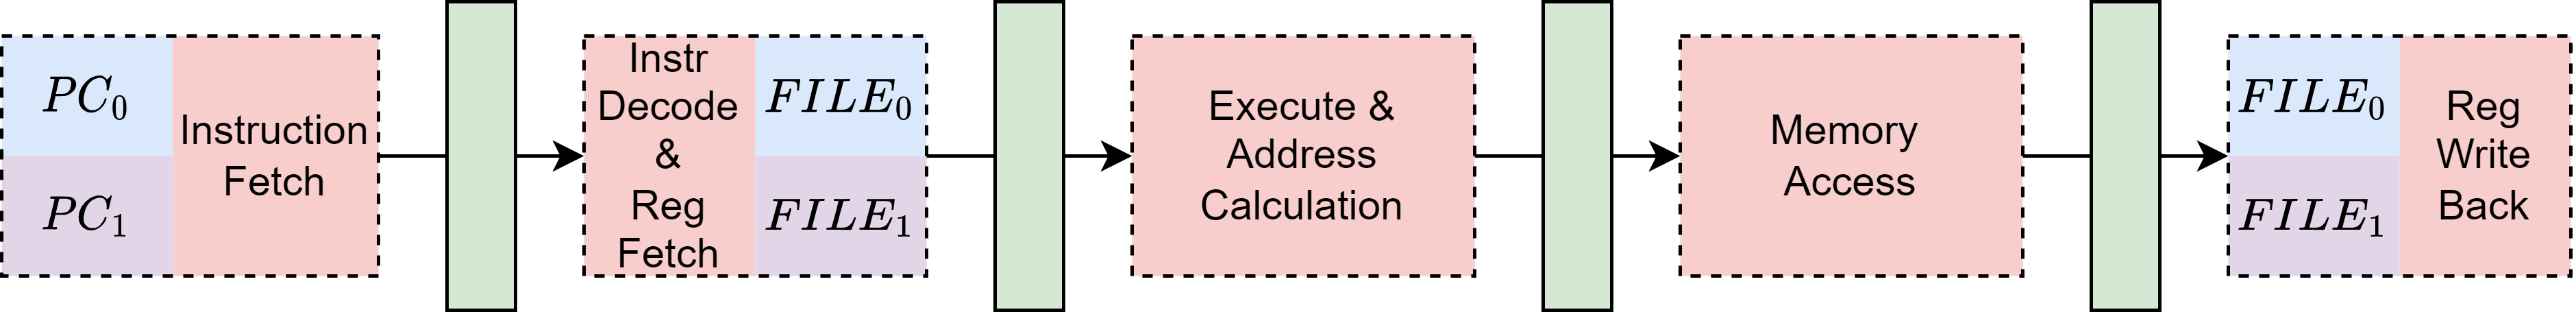
\includegraphics[width=.9\textwidth]{pipelining/images/simultaneous_multithreading.drawio.png}
\end{center}
We can eliminate stalls by interleaving the instructions of independent programs. 
\begin{itemize}
    \item Maintain two program counters for two programs, two sets of registers. Alternate between instructions from each program.
    \item No dependencies between adjacent stages, less forwarding, less complex instruction decode and control required.
    \item Each program sees half the clock frequency.
\end{itemize}

\section{Pipelining Roundup}
Pipelining offers increased throughput without much added hardware complexity by allowing execution stages to run in parallel as a pipeline.
\begin{itemize}
    \item Simple 5 stage pipeline can run at $5 \to 9$GHz
    \item Limited by critical path through slowest pipeline stage
    \item Clock period is $330ps \approx 10$ gate delays at $3GHz$ ($3 \to 5$ FO4 for latches, $5\to8$ FO4 for work).
    \item Memory access needs to be done in $5\to8$ FO4 delays (large constraint).
\end{itemize}

\begin{sidenotebox}{FO4 Delays}
    The gate delay of a component with a fan-out (gate inputs driven by a gate's output) of 4.
\end{sidenotebox}